\section{Durchf\"{u}hrung}
\begin{enumerate}
\item
\label{par:a}
Mithilfe eines Ringmodulators wird ein amplitudenmoduliertes Signal erzeugt. Die dabei entstehende Schwebung wird anschließend mit einem
Oszilloskop visualisiert. Auch wird mit Hilfe eines Frequenzanalysators das Frequenzspektrum des erzeugten Signals sichtbar gemacht.

\item
\label{par:b}
Aufgabenteil (a) wird mit einer Diode zur Modulation wiederholt und die selben Signalseigenschaften untersucht.
Außerdem wird der Modulationsgrad m aus dem Signal gewonnen und gezeigt, dass zusätzlich Oberwellen von $\omega_\text{T}$ auftreten.

\item
\label{par:c}
Mithilfe einer Schaltung gemäß Abbildung \ref{Abb14} und eines Multimeters wird die Proportionalität am Ausgang X mit dem Cosinus der Phase zwischen 
Ein- und Ausgang eines Ringmodulators gezeigt.

\begin{figure}
	\centering
	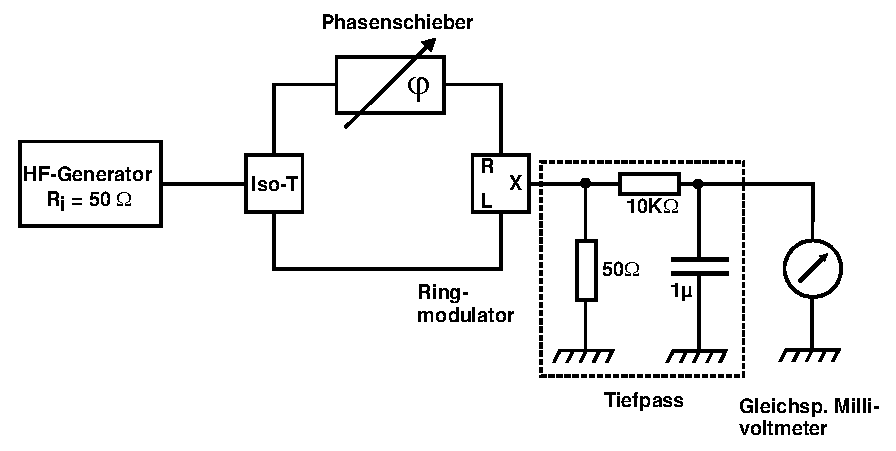
\includegraphics[width=\textwidth]{img/Abb14.pdf}
	\caption{Schaltung zum Aufnehmen der Beziehung zwischen Gleichspannung und Phase der Wechselspannung. \cite{FP}}
	\label{Abb14}
\end{figure}

\item
\label{par:d}
Das Multimeter aus \ref{par:d} wird durch ein Oszilloskop ersetzt und das demodulierte Signal sichtbar gemacht.

\item
\label{par:e}
Mit Hilfe einer Gleichrichterdiode wird ein amplitudenmoduliertes Signal demoduliert.
Außerdem wird die Zeitabhängigkeit vor und hinter dem Tiefpass dargestellt.

\item
\label{par:f}
Es wird ein frequenzmoduliertes Signal erzeugt, welches auf einem Oszilloskop dargestellt wird. Anschließend wird der Frequenzhub und
der Modulationsgrad ermittelt und das Frequenzspektrum untersucht.

\item
\label{par:g}
Abschließend wird ein frequenzmoduliertes Signal demoduliert und das Ergebnis visualisiert.
\end{enumerate}
